% Created by tikzDevice version 0.12.3.1 on 2022-04-28 16:23:30
% !TEX encoding = UTF-8 Unicode
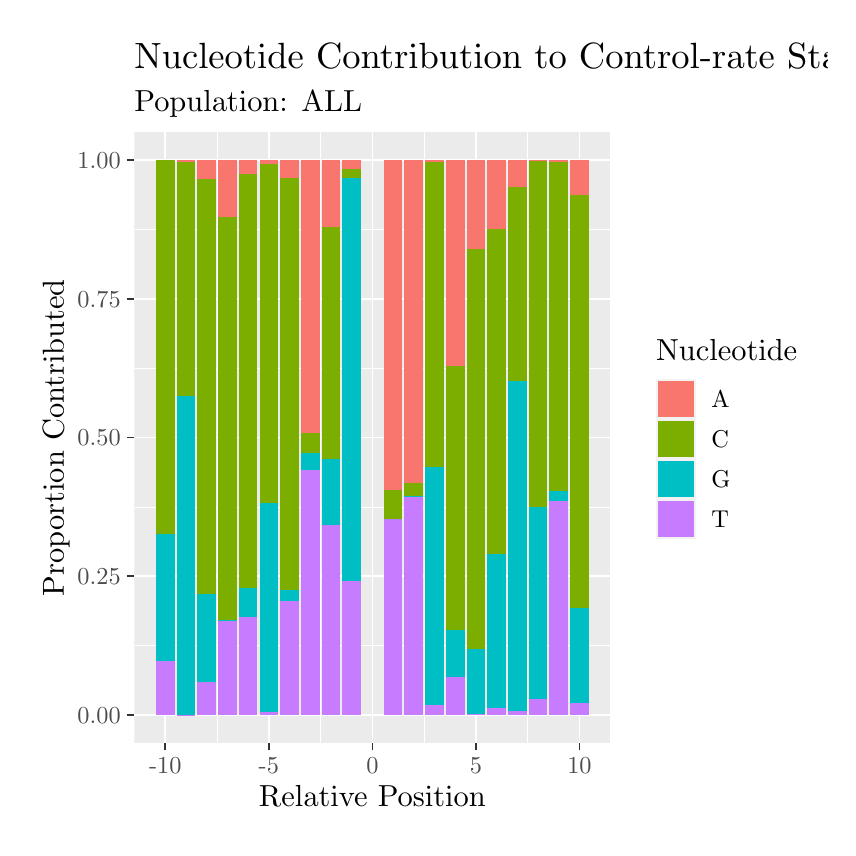
\begin{tikzpicture}[x=1pt,y=1pt]
\definecolor{fillColor}{RGB}{255,255,255}
\path[use as bounding box,fill=fillColor,fill opacity=0.00] (0,0) rectangle (289.08,289.08);
\begin{scope}
\path[clip] (  0.00,  0.00) rectangle (289.08,289.08);
\definecolor{drawColor}{RGB}{255,255,255}
\definecolor{fillColor}{RGB}{255,255,255}

\path[draw=drawColor,line width= 0.6pt,line join=round,line cap=round,fill=fillColor] (  0.00,  0.00) rectangle (289.08,289.08);
\end{scope}
\begin{scope}
\path[clip] ( 38.56, 30.69) rectangle (210.56,251.21);
\definecolor{fillColor}{gray}{0.92}

\path[fill=fillColor] ( 38.56, 30.69) rectangle (210.56,251.21);
\definecolor{drawColor}{RGB}{255,255,255}

\path[draw=drawColor,line width= 0.3pt,line join=round] ( 38.56, 65.77) --
	(210.56, 65.77);

\path[draw=drawColor,line width= 0.3pt,line join=round] ( 38.56,115.89) --
	(210.56,115.89);

\path[draw=drawColor,line width= 0.3pt,line join=round] ( 38.56,166.01) --
	(210.56,166.01);

\path[draw=drawColor,line width= 0.3pt,line join=round] ( 38.56,216.13) --
	(210.56,216.13);

\path[draw=drawColor,line width= 0.3pt,line join=round] ( 68.45, 30.69) --
	( 68.45,251.21);

\path[draw=drawColor,line width= 0.3pt,line join=round] (105.85, 30.69) --
	(105.85,251.21);

\path[draw=drawColor,line width= 0.3pt,line join=round] (143.26, 30.69) --
	(143.26,251.21);

\path[draw=drawColor,line width= 0.3pt,line join=round] (180.67, 30.69) --
	(180.67,251.21);

\path[draw=drawColor,line width= 0.6pt,line join=round] ( 38.56, 40.71) --
	(210.56, 40.71);

\path[draw=drawColor,line width= 0.6pt,line join=round] ( 38.56, 90.83) --
	(210.56, 90.83);

\path[draw=drawColor,line width= 0.6pt,line join=round] ( 38.56,140.95) --
	(210.56,140.95);

\path[draw=drawColor,line width= 0.6pt,line join=round] ( 38.56,191.07) --
	(210.56,191.07);

\path[draw=drawColor,line width= 0.6pt,line join=round] ( 38.56,241.18) --
	(210.56,241.18);

\path[draw=drawColor,line width= 0.6pt,line join=round] ( 49.74, 30.69) --
	( 49.74,251.21);

\path[draw=drawColor,line width= 0.6pt,line join=round] ( 87.15, 30.69) --
	( 87.15,251.21);

\path[draw=drawColor,line width= 0.6pt,line join=round] (124.56, 30.69) --
	(124.56,251.21);

\path[draw=drawColor,line width= 0.6pt,line join=round] (161.97, 30.69) --
	(161.97,251.21);

\path[draw=drawColor,line width= 0.6pt,line join=round] (199.38, 30.69) --
	(199.38,251.21);
\definecolor{fillColor}{RGB}{248,118,109}

\path[fill=fillColor] ( 46.37,241.17) rectangle ( 53.11,241.18);
\definecolor{fillColor}{RGB}{124,174,0}

\path[fill=fillColor] ( 46.37,105.98) rectangle ( 53.11,241.17);
\definecolor{fillColor}{RGB}{0,191,196}

\path[fill=fillColor] ( 46.37, 60.08) rectangle ( 53.11,105.98);
\definecolor{fillColor}{RGB}{199,124,255}

\path[fill=fillColor] ( 46.37, 40.71) rectangle ( 53.11, 60.08);
\definecolor{fillColor}{RGB}{248,118,109}

\path[fill=fillColor] ( 53.86,240.53) rectangle ( 60.59,241.18);
\definecolor{fillColor}{RGB}{124,174,0}

\path[fill=fillColor] ( 53.86,155.95) rectangle ( 60.59,240.53);
\definecolor{fillColor}{RGB}{199,124,255}

\path[fill=fillColor] ( 53.86, 40.71) rectangle ( 60.59, 40.73);
\definecolor{fillColor}{RGB}{0,191,196}

\path[fill=fillColor] ( 53.86, 40.73) rectangle ( 60.59,155.95);
\definecolor{fillColor}{RGB}{248,118,109}

\path[fill=fillColor] ( 61.34,234.56) rectangle ( 68.07,241.18);
\definecolor{fillColor}{RGB}{124,174,0}

\path[fill=fillColor] ( 61.34, 84.40) rectangle ( 68.07,234.56);
\definecolor{fillColor}{RGB}{0,191,196}

\path[fill=fillColor] ( 61.34, 52.74) rectangle ( 68.07, 84.40);
\definecolor{fillColor}{RGB}{199,124,255}

\path[fill=fillColor] ( 61.34, 40.71) rectangle ( 68.07, 52.74);
\definecolor{fillColor}{RGB}{248,118,109}

\path[fill=fillColor] ( 68.82,220.66) rectangle ( 75.55,241.18);
\definecolor{fillColor}{RGB}{124,174,0}

\path[fill=fillColor] ( 68.82, 74.93) rectangle ( 75.55,220.66);
\definecolor{fillColor}{RGB}{199,124,255}

\path[fill=fillColor] ( 68.82, 40.71) rectangle ( 75.55, 74.86);
\definecolor{fillColor}{RGB}{0,191,196}

\path[fill=fillColor] ( 68.82, 74.86) rectangle ( 75.55, 74.93);
\definecolor{fillColor}{RGB}{248,118,109}

\path[fill=fillColor] ( 76.30,236.36) rectangle ( 83.04,241.18);
\definecolor{fillColor}{RGB}{124,174,0}

\path[fill=fillColor] ( 76.30, 86.57) rectangle ( 83.04,236.36);
\definecolor{fillColor}{RGB}{199,124,255}

\path[fill=fillColor] ( 76.30, 40.71) rectangle ( 83.04, 76.30);
\definecolor{fillColor}{RGB}{0,191,196}

\path[fill=fillColor] ( 76.30, 76.30) rectangle ( 83.04, 86.57);
\definecolor{fillColor}{RGB}{248,118,109}

\path[fill=fillColor] ( 83.78,239.98) rectangle ( 90.52,241.18);
\definecolor{fillColor}{RGB}{124,174,0}

\path[fill=fillColor] ( 83.78,117.39) rectangle ( 90.52,239.98);
\definecolor{fillColor}{RGB}{0,191,196}

\path[fill=fillColor] ( 83.78, 41.87) rectangle ( 90.52,117.39);
\definecolor{fillColor}{RGB}{199,124,255}

\path[fill=fillColor] ( 83.78, 40.71) rectangle ( 90.52, 41.87);
\definecolor{fillColor}{RGB}{248,118,109}

\path[fill=fillColor] ( 91.27,234.90) rectangle ( 98.00,241.18);
\definecolor{fillColor}{RGB}{124,174,0}

\path[fill=fillColor] ( 91.27, 85.73) rectangle ( 98.00,234.90);
\definecolor{fillColor}{RGB}{199,124,255}

\path[fill=fillColor] ( 91.27, 40.71) rectangle ( 98.00, 81.99);
\definecolor{fillColor}{RGB}{0,191,196}

\path[fill=fillColor] ( 91.27, 81.99) rectangle ( 98.00, 85.73);
\definecolor{fillColor}{RGB}{248,118,109}

\path[fill=fillColor] ( 98.75,142.58) rectangle (105.48,241.18);
\definecolor{fillColor}{RGB}{124,174,0}

\path[fill=fillColor] ( 98.75,135.45) rectangle (105.48,142.58);
\definecolor{fillColor}{RGB}{0,191,196}

\path[fill=fillColor] ( 98.75,129.07) rectangle (105.48,135.45);
\definecolor{fillColor}{RGB}{199,124,255}

\path[fill=fillColor] ( 98.75, 40.71) rectangle (105.48,129.07);
\definecolor{fillColor}{RGB}{248,118,109}

\path[fill=fillColor] (106.23,216.93) rectangle (112.96,241.18);
\definecolor{fillColor}{RGB}{124,174,0}

\path[fill=fillColor] (106.23,133.09) rectangle (112.96,216.93);
\definecolor{fillColor}{RGB}{199,124,255}

\path[fill=fillColor] (106.23, 40.71) rectangle (112.96,109.48);
\definecolor{fillColor}{RGB}{0,191,196}

\path[fill=fillColor] (106.23,109.48) rectangle (112.96,133.09);
\definecolor{fillColor}{RGB}{248,118,109}

\path[fill=fillColor] (113.71,237.96) rectangle (120.44,241.18);
\definecolor{fillColor}{RGB}{124,174,0}

\path[fill=fillColor] (113.71,234.81) rectangle (120.44,237.96);
\definecolor{fillColor}{RGB}{199,124,255}

\path[fill=fillColor] (113.71, 40.71) rectangle (120.44, 88.98);
\definecolor{fillColor}{RGB}{0,191,196}

\path[fill=fillColor] (113.71, 88.98) rectangle (120.44,234.81);
\definecolor{fillColor}{RGB}{248,118,109}

\path[fill=fillColor] (128.67,121.93) rectangle (135.41,241.18);
\definecolor{fillColor}{RGB}{124,174,0}

\path[fill=fillColor] (128.67,111.68) rectangle (135.41,121.93);
\definecolor{fillColor}{RGB}{199,124,255}

\path[fill=fillColor] (128.67, 40.71) rectangle (135.41,111.68);
\definecolor{fillColor}{RGB}{0,191,196}

\path[fill=fillColor] (128.67,111.68) rectangle (135.41,111.68);
\definecolor{fillColor}{RGB}{248,118,109}

\path[fill=fillColor] (136.16,124.68) rectangle (142.89,241.18);
\definecolor{fillColor}{RGB}{124,174,0}

\path[fill=fillColor] (136.16,119.89) rectangle (142.89,124.68);
\definecolor{fillColor}{RGB}{199,124,255}

\path[fill=fillColor] (136.16, 40.71) rectangle (142.89,119.44);
\definecolor{fillColor}{RGB}{0,191,196}

\path[fill=fillColor] (136.16,119.44) rectangle (142.89,119.89);
\definecolor{fillColor}{RGB}{248,118,109}

\path[fill=fillColor] (143.64,240.36) rectangle (150.37,241.18);
\definecolor{fillColor}{RGB}{124,174,0}

\path[fill=fillColor] (143.64,130.32) rectangle (150.37,240.36);
\definecolor{fillColor}{RGB}{199,124,255}

\path[fill=fillColor] (143.64, 40.71) rectangle (150.37, 44.50);
\definecolor{fillColor}{RGB}{0,191,196}

\path[fill=fillColor] (143.64, 44.50) rectangle (150.37,130.32);
\definecolor{fillColor}{RGB}{248,118,109}

\path[fill=fillColor] (151.12,166.70) rectangle (157.85,241.18);
\definecolor{fillColor}{RGB}{124,174,0}

\path[fill=fillColor] (151.12, 71.58) rectangle (157.85,166.70);
\definecolor{fillColor}{RGB}{0,191,196}

\path[fill=fillColor] (151.12, 54.55) rectangle (157.85, 71.58);
\definecolor{fillColor}{RGB}{199,124,255}

\path[fill=fillColor] (151.12, 40.71) rectangle (157.85, 54.55);
\definecolor{fillColor}{RGB}{248,118,109}

\path[fill=fillColor] (158.60,208.97) rectangle (165.34,241.18);
\definecolor{fillColor}{RGB}{124,174,0}

\path[fill=fillColor] (158.60, 64.69) rectangle (165.34,208.97);
\definecolor{fillColor}{RGB}{0,191,196}

\path[fill=fillColor] (158.60, 41.06) rectangle (165.34, 64.69);
\definecolor{fillColor}{RGB}{199,124,255}

\path[fill=fillColor] (158.60, 40.71) rectangle (165.34, 41.06);
\definecolor{fillColor}{RGB}{248,118,109}

\path[fill=fillColor] (166.08,216.18) rectangle (172.82,241.18);
\definecolor{fillColor}{RGB}{124,174,0}

\path[fill=fillColor] (166.08, 99.06) rectangle (172.82,216.18);
\definecolor{fillColor}{RGB}{0,191,196}

\path[fill=fillColor] (166.08, 43.21) rectangle (172.82, 99.06);
\definecolor{fillColor}{RGB}{199,124,255}

\path[fill=fillColor] (166.08, 40.71) rectangle (172.82, 43.21);
\definecolor{fillColor}{RGB}{248,118,109}

\path[fill=fillColor] (173.57,231.45) rectangle (180.30,241.18);
\definecolor{fillColor}{RGB}{124,174,0}

\path[fill=fillColor] (173.57,161.26) rectangle (180.30,231.45);
\definecolor{fillColor}{RGB}{199,124,255}

\path[fill=fillColor] (173.57, 40.71) rectangle (180.30, 41.98);
\definecolor{fillColor}{RGB}{0,191,196}

\path[fill=fillColor] (173.57, 41.98) rectangle (180.30,161.26);
\definecolor{fillColor}{RGB}{248,118,109}

\path[fill=fillColor] (181.05,241.01) rectangle (187.78,241.18);
\definecolor{fillColor}{RGB}{124,174,0}

\path[fill=fillColor] (181.05,116.00) rectangle (187.78,241.01);
\definecolor{fillColor}{RGB}{199,124,255}

\path[fill=fillColor] (181.05, 40.71) rectangle (187.78, 46.58);
\definecolor{fillColor}{RGB}{0,191,196}

\path[fill=fillColor] (181.05, 46.58) rectangle (187.78,116.00);
\definecolor{fillColor}{RGB}{248,118,109}

\path[fill=fillColor] (188.53,240.49) rectangle (195.26,241.18);
\definecolor{fillColor}{RGB}{124,174,0}

\path[fill=fillColor] (188.53,121.66) rectangle (195.26,240.49);
\definecolor{fillColor}{RGB}{0,191,196}

\path[fill=fillColor] (188.53,118.14) rectangle (195.26,121.66);
\definecolor{fillColor}{RGB}{199,124,255}

\path[fill=fillColor] (188.53, 40.71) rectangle (195.26,118.14);
\definecolor{fillColor}{RGB}{248,118,109}

\path[fill=fillColor] (196.01,228.48) rectangle (202.75,241.18);
\definecolor{fillColor}{RGB}{124,174,0}

\path[fill=fillColor] (196.01, 79.51) rectangle (202.75,228.48);
\definecolor{fillColor}{RGB}{199,124,255}

\path[fill=fillColor] (196.01, 40.71) rectangle (202.75, 44.93);
\definecolor{fillColor}{RGB}{0,191,196}

\path[fill=fillColor] (196.01, 44.93) rectangle (202.75, 79.51);
\end{scope}
\begin{scope}
\path[clip] (  0.00,  0.00) rectangle (289.08,289.08);
\definecolor{drawColor}{gray}{0.30}

\node[text=drawColor,anchor=base east,inner sep=0pt, outer sep=0pt, scale=  0.88] at ( 33.61, 37.68) {0.00};

\node[text=drawColor,anchor=base east,inner sep=0pt, outer sep=0pt, scale=  0.88] at ( 33.61, 87.80) {0.25};

\node[text=drawColor,anchor=base east,inner sep=0pt, outer sep=0pt, scale=  0.88] at ( 33.61,137.92) {0.50};

\node[text=drawColor,anchor=base east,inner sep=0pt, outer sep=0pt, scale=  0.88] at ( 33.61,188.04) {0.75};

\node[text=drawColor,anchor=base east,inner sep=0pt, outer sep=0pt, scale=  0.88] at ( 33.61,238.15) {1.00};
\end{scope}
\begin{scope}
\path[clip] (  0.00,  0.00) rectangle (289.08,289.08);
\definecolor{drawColor}{gray}{0.20}

\path[draw=drawColor,line width= 0.6pt,line join=round] ( 35.81, 40.71) --
	( 38.56, 40.71);

\path[draw=drawColor,line width= 0.6pt,line join=round] ( 35.81, 90.83) --
	( 38.56, 90.83);

\path[draw=drawColor,line width= 0.6pt,line join=round] ( 35.81,140.95) --
	( 38.56,140.95);

\path[draw=drawColor,line width= 0.6pt,line join=round] ( 35.81,191.07) --
	( 38.56,191.07);

\path[draw=drawColor,line width= 0.6pt,line join=round] ( 35.81,241.18) --
	( 38.56,241.18);
\end{scope}
\begin{scope}
\path[clip] (  0.00,  0.00) rectangle (289.08,289.08);
\definecolor{drawColor}{gray}{0.20}

\path[draw=drawColor,line width= 0.6pt,line join=round] ( 49.74, 27.94) --
	( 49.74, 30.69);

\path[draw=drawColor,line width= 0.6pt,line join=round] ( 87.15, 27.94) --
	( 87.15, 30.69);

\path[draw=drawColor,line width= 0.6pt,line join=round] (124.56, 27.94) --
	(124.56, 30.69);

\path[draw=drawColor,line width= 0.6pt,line join=round] (161.97, 27.94) --
	(161.97, 30.69);

\path[draw=drawColor,line width= 0.6pt,line join=round] (199.38, 27.94) --
	(199.38, 30.69);
\end{scope}
\begin{scope}
\path[clip] (  0.00,  0.00) rectangle (289.08,289.08);
\definecolor{drawColor}{gray}{0.30}

\node[text=drawColor,anchor=base,inner sep=0pt, outer sep=0pt, scale=  0.88] at ( 49.74, 19.68) {-10};

\node[text=drawColor,anchor=base,inner sep=0pt, outer sep=0pt, scale=  0.88] at ( 87.15, 19.68) {-5};

\node[text=drawColor,anchor=base,inner sep=0pt, outer sep=0pt, scale=  0.88] at (124.56, 19.68) {0};

\node[text=drawColor,anchor=base,inner sep=0pt, outer sep=0pt, scale=  0.88] at (161.97, 19.68) {5};

\node[text=drawColor,anchor=base,inner sep=0pt, outer sep=0pt, scale=  0.88] at (199.38, 19.68) {10};
\end{scope}
\begin{scope}
\path[clip] (  0.00,  0.00) rectangle (289.08,289.08);
\definecolor{drawColor}{RGB}{0,0,0}

\node[text=drawColor,anchor=base,inner sep=0pt, outer sep=0pt, scale=  1.10] at (124.56,  7.64) {Relative Position};
\end{scope}
\begin{scope}
\path[clip] (  0.00,  0.00) rectangle (289.08,289.08);
\definecolor{drawColor}{RGB}{0,0,0}

\node[text=drawColor,rotate= 90.00,anchor=base,inner sep=0pt, outer sep=0pt, scale=  1.10] at ( 13.08,140.95) {Proportion Contributed};
\end{scope}
\begin{scope}
\path[clip] (  0.00,  0.00) rectangle (289.08,289.08);
\definecolor{fillColor}{RGB}{255,255,255}

\path[fill=fillColor] (221.56, 98.93) rectangle (283.58,182.96);
\end{scope}
\begin{scope}
\path[clip] (  0.00,  0.00) rectangle (289.08,289.08);
\definecolor{drawColor}{RGB}{0,0,0}

\node[text=drawColor,anchor=base west,inner sep=0pt, outer sep=0pt, scale=  1.10] at (227.06,168.82) {Nucleotide};
\end{scope}
\begin{scope}
\path[clip] (  0.00,  0.00) rectangle (289.08,289.08);
\definecolor{fillColor}{gray}{0.95}

\path[fill=fillColor] (227.06,147.79) rectangle (241.52,162.25);
\end{scope}
\begin{scope}
\path[clip] (  0.00,  0.00) rectangle (289.08,289.08);
\definecolor{fillColor}{RGB}{248,118,109}

\path[fill=fillColor] (227.78,148.51) rectangle (240.81,161.54);
\end{scope}
\begin{scope}
\path[clip] (  0.00,  0.00) rectangle (289.08,289.08);
\definecolor{fillColor}{gray}{0.95}

\path[fill=fillColor] (227.06,133.34) rectangle (241.52,147.79);
\end{scope}
\begin{scope}
\path[clip] (  0.00,  0.00) rectangle (289.08,289.08);
\definecolor{fillColor}{RGB}{124,174,0}

\path[fill=fillColor] (227.78,134.05) rectangle (240.81,147.08);
\end{scope}
\begin{scope}
\path[clip] (  0.00,  0.00) rectangle (289.08,289.08);
\definecolor{fillColor}{gray}{0.95}

\path[fill=fillColor] (227.06,118.89) rectangle (241.52,133.34);
\end{scope}
\begin{scope}
\path[clip] (  0.00,  0.00) rectangle (289.08,289.08);
\definecolor{fillColor}{RGB}{0,191,196}

\path[fill=fillColor] (227.78,119.60) rectangle (240.81,132.63);
\end{scope}
\begin{scope}
\path[clip] (  0.00,  0.00) rectangle (289.08,289.08);
\definecolor{fillColor}{gray}{0.95}

\path[fill=fillColor] (227.06,104.43) rectangle (241.52,118.89);
\end{scope}
\begin{scope}
\path[clip] (  0.00,  0.00) rectangle (289.08,289.08);
\definecolor{fillColor}{RGB}{199,124,255}

\path[fill=fillColor] (227.78,105.14) rectangle (240.81,118.17);
\end{scope}
\begin{scope}
\path[clip] (  0.00,  0.00) rectangle (289.08,289.08);
\definecolor{drawColor}{RGB}{0,0,0}

\node[text=drawColor,anchor=base west,inner sep=0pt, outer sep=0pt, scale=  0.88] at (247.02,151.99) {A};
\end{scope}
\begin{scope}
\path[clip] (  0.00,  0.00) rectangle (289.08,289.08);
\definecolor{drawColor}{RGB}{0,0,0}

\node[text=drawColor,anchor=base west,inner sep=0pt, outer sep=0pt, scale=  0.88] at (247.02,137.54) {C};
\end{scope}
\begin{scope}
\path[clip] (  0.00,  0.00) rectangle (289.08,289.08);
\definecolor{drawColor}{RGB}{0,0,0}

\node[text=drawColor,anchor=base west,inner sep=0pt, outer sep=0pt, scale=  0.88] at (247.02,123.08) {G};
\end{scope}
\begin{scope}
\path[clip] (  0.00,  0.00) rectangle (289.08,289.08);
\definecolor{drawColor}{RGB}{0,0,0}

\node[text=drawColor,anchor=base west,inner sep=0pt, outer sep=0pt, scale=  0.88] at (247.02,108.63) {T};
\end{scope}
\begin{scope}
\path[clip] (  0.00,  0.00) rectangle (289.08,289.08);
\definecolor{drawColor}{RGB}{0,0,0}

\node[text=drawColor,anchor=base west,inner sep=0pt, outer sep=0pt, scale=  1.10] at ( 38.56,258.85) {Population: ALL};
\end{scope}
\begin{scope}
\path[clip] (  0.00,  0.00) rectangle (289.08,289.08);
\definecolor{drawColor}{RGB}{0,0,0}

\node[text=drawColor,anchor=base west,inner sep=0pt, outer sep=0pt, scale=  1.32] at ( 38.56,274.49) {Nucleotide Contribution to Control-rate Statistic: GC-CG};
\end{scope}
\end{tikzpicture}
